\documentclass[11pt]{article}
\usepackage[T1]{fontenc}
\usepackage{lmodern}
\usepackage[margin=1in]{geometry}
\usepackage{amsmath,amssymb,amsthm,mathtools}
\usepackage{booktabs,microtype}
\usepackage[colorlinks=true,linkcolor=blue,citecolor=blue,urlcolor=blue]{hyperref}
\usepackage{enumitem}
\usepackage{graphicx}
\hypersetup{pdftitle={Uniform rectangular laws for symplectic compressions},pdfauthor={Research note prepared for Vladimir Reshetnikov},pdfsubject={Complete proofs of uniform rank laws and residual dependence}}

\newtheorem{theorem}{Theorem}[section]
\newtheorem{proposition}[theorem]{Proposition}
\newtheorem{lemma}[theorem]{Lemma}
\newtheorem{corollary}[theorem]{Corollary}
\theoremstyle{definition}
\newtheorem{definition}[theorem]{Definition}
\theoremstyle{remark}
\newtheorem{remark}[theorem]{Remark}

\newcommand{\F}{\mathbb F}
\newcommand{\N}{\mathbb N}
\newcommand{\Pp}{\mathbb P}
\newcommand{\E}{\mathbb E}
\newcommand{\Law}{\mathcal L}
\newcommand{\TV}{d_{\mathrm{TV}}}
\newcommand{\Mat}{\operatorname{Mat}}
\newcommand{\Alt}{\operatorname{Alt}}
\newcommand{\Sp}{\operatorname{Sp}}
\newcommand{\GL}{\operatorname{GL}}
\newcommand{\rank}{\operatorname{rank}}
\newcommand{\rad}{\operatorname{rad}}
\newcommand{\nul}{\operatorname{nul}}
\newcommand{\Emb}{\mathcal E}
\newcommand{\gb}[2]{\begin{bmatrix}#1\\#2\end{bmatrix}_{q}}
\newcommand{\normone}[1]{\left\|#1\right\|_1}
\newcommand{\abs}[1]{\left|#1\right|}
\newcommand{\tr}{\mathsf T}

\title{Uniform rectangular laws for symplectic compressions:\\
rank blindness and residual dependence}
\author{\small Research note prepared for Vladimir Reshetnikov}
\date{November 27, 2026}

\begin{document}
\maketitle

\begin{abstract}
Consider a rectangular block of a uniformly random symplectic matrix over a finite field, when the source and target frames are nondegenerate and their dimensions add to the ambient dimension. We prove first-order expansions for its rank law, for the nullity of its quadratic residual form, and for the dependence between ordinary and residual nullities. The error terms are uniform in the aspect ratio, including a fixed positive gap between the two dimensions. If the block has size $a\times b$, with $a\ge b$ even, its rank law differs from that of independent uniform entries by an explicit constant times $q^{-a}$, with error $O_q(q^{-a-b})$. In contrast, the distance between the full matrix laws tends to the same positive infinite-product constant for every way in which both dimensions grow. We also identify the first nonzero correction to independence between the two nullities as an explicit tensor product of signed measures. The results are unconditional. They extend the symplectic-compression branch of the supplied GRH research article, resolve its stated fixed-gap case, and separate the new uniform estimates from the inherited exact counting formulas.
\end{abstract}

\tableofcontents

\section{The question and the contribution}

The supplied research program studies both consequences of Dirichlet GRH and methods that can be transferred from the proof to other settings. Its section on spanning, frames, and matrix statistics contains an exact finite law for symplectic compressions and several limiting regimes \cite{ProveIt}. The present paper develops that branch. Its subject is finite linear algebra and probability; none of the proofs below assumes a statement about zeros of an $L$-function.

The phenomenon is easy to describe. A block cut from a random symplectic matrix has dependent entries. Its rank may nevertheless be almost indistinguishable from the rank of a matrix with independent uniform entries. The full block retains a detectable constraint, visible through a second matrix obtained by substituting the block into the symplectic form. The question is whether this separation persists uniformly as the dimensions grow in different proportions, and what the exact leading errors are.

\subsection{The pinned source and the novelty boundary}

Our comparison is with the \texttt{VladimirReshetnikov/ProveIt} repository at the fixed commit
\begin{center}\small
\texttt{497c1844e71393df41914f5b783d5dc9a618eb61}.
\end{center}
The relevant source is
\nolinkurl{Analysis/GeneralizedRiemannHypothesis/Article/sections/spn.tex}.
The following source results are used as context and are rederived where needed:

\begin{itemize}[leftmargin=1.6em]
\item \texttt{spn:thm:balanced} gives the exact residual likelihood and the optimal singularity test for every complementary pair of nondegenerate frames.
\item \texttt{spn:thm:nondeg-blind} gives the positive full-matrix limit when the block becomes increasingly tall, together with an $O_q(q^{b-a})$ bound for the rank discrepancy.
\item \texttt{spn:thm:square-block} and \texttt{spn:thm:defect-universality} give the first-order marginal laws for square blocks.
\item \texttt{spn:q:symplectic} explicitly asks for the remaining growing regimes; it records only a lower bound when $a-b$ is fixed and positive.
\end{itemize}

The new statements here are the expansions uniform over every rectangular gap, the sharp $q^{-a}$ rank rate with an $O_q(q^{-a-b})$ error, the corresponding finite-product correction to the full distance, and the first-order joint independence law. The exact likelihood, the classical matrix-nullity distributions, and the square specialization of the marginal expansions are not claimed as new. Classical comparison results for independent-entry rectangular and alternating matrices are treated by Fulman and Goldstein \cite{FulmanGoldstein}. Exact nondegenerate-subspace enumeration has further antecedents in De Boeck and Van de Voorde \cite{DeBoeckVanDeVoorde}. Our proofs include the elementary counting and quantitative inversion needed for the present dependent matrix model; the contribution concerns the uniform statistical laws and their corrections.

These statements are new relative to the pinned source. The cited literature and targeted searches did not identify the same uniform symplectic-compression or joint expansions; this is a bounded assessment of novelty, not a certification of priority across all literature.

\section{Definitions and main results}\label{sec:main}

Fix a prime power $q$. Throughout, an alternating matrix has zero diagonal and satisfies $H^{\tr}=-H$; the diagonal condition is retained in characteristic two. For every positive even integer $r$, let $J_r$ be a fixed nonsingular alternating $r\times r$ matrix.

Let $a\ge b\ge2$ be even, and equip
\[
 V=(\F_q^a,J_a)\perp(\F_q^b,J_b)
\]
with its orthogonal direct-sum form. If $g$ is uniform in $\Sp(V)$, write its last $b$ columns as
\begin{equation}\label{eq:model}
 g\begin{pmatrix}0\\I_b\end{pmatrix}
 =\begin{pmatrix}A\\B\end{pmatrix},
 \qquad A\in\Mat_{a,b}(\F_q),\quad B\in\Mat_b(\F_q).
\end{equation}
Thus
\begin{equation}\label{eq:gram-condition}
 A^{\tr}J_aA+B^{\tr}J_bB=J_b.
\end{equation}
Let $U$ be uniform on $\Mat_{a,b}(\F_q)$, and let $T$ be uniform on the additive group $\Alt_b(\F_q)$. Define
\[
 N(M)=\dim\ker M,\qquad
 \Lambda(M)=J_b-M^{\tr}J_aM,\qquad D(M)=\dim\ker\Lambda(M).
\]
In particular, $D(M)$ is even. Put
\begin{equation}\label{eq:parameters}
 d=a-b,\qquad \tau=q^{-b},\qquad \sigma=q^{-a}=\tau q^{-d}.
\end{equation}
All constants implicit in $O_q(\cdot)$ depend only on $q$, uniformly in $a,b,d$.

For a signed measure on a countable set, $\normone{\mu}$ is the sum of the absolute masses. For probability measures,
\[
 \TV(\mu,\nu)=\tfrac12\normone{\mu-\nu}.
\]
We also write $\TV(X,Y)$ for the distance between the laws of two random variables. Tensor products below may involve signed measures.

\subsection{Infinite products and signed correction laws}

Set
\begin{gather*}
 \gamma_r=\prod_{i=1}^r(1-q^{-i}),\qquad
 \eta_r=\prod_{i=1}^r(1-q^{-2i}),\qquad
 \theta_r=\prod_{i=1}^r(1-q^{-(2i-1)}),\\
 \gamma=\gamma_\infty,\qquad \eta=\eta_\infty,\qquad
 \theta=\theta_\infty,
 \qquad \gamma=\eta\theta.
\end{gather*}
Empty products equal one. Define probability measures on $\N_0$ by
\begin{equation}\label{eq:limit-laws}
 \pi_d(k)=\frac{\gamma q^{-k(k+d)}}{\gamma_k\gamma_{k+d}},\qquad
 \lambda(2k)=\frac{\theta q^{-k(2k-1)}}{\gamma_{2k}},\qquad
 \lambda(2k+1)=0.
\end{equation}
Their normalization and moments are proved below. The signed measures that describe the corrections are
\begin{equation}\label{eq:signed-laws}
 \xi_d(k)=\frac{1+q^{-d}-q^k}{q-1}\pi_d(k),\qquad
 \zeta(k)=\frac{q+1-q^k}{q^2-1}\lambda(k).
\end{equation}
Both have total mass zero. Their only strictly positive mass is at zero, and
\begin{equation}\label{eq:signed-norms}
 \normone{\xi_d}=\frac{2q^{-d}\pi_d(0)}{q-1},\qquad
 \normone{\zeta}=\frac{2q\theta}{q^2-1}.
\end{equation}
At $q=2,d=0$, the mass $\xi_0(1)$ is zero; this does not change these formulas.

\subsection{The uniform marginal laws}

\begin{theorem}[Uniform nullity expansions]\label{thm:marginal}
For every prime power $q$ and every positive even $a\ge b$,
\begin{align}
 \normone{\Law(N(A))-\Law(N(U))-\tau\xi_d}
 &=O_q(\sigma\tau),\label{eq:rank-signed}\\
 \normone{\Law(D(U))-\Law(\dim\ker T)-\sigma\zeta}
 &=O_q(\sigma\tau).\label{eq:defect-signed}
\end{align}
Consequently,
\begin{align}
 \TV(\rank A,\rank U)
 &=\frac{\gamma}{(q-1)\gamma_d}\,q^{-a}
   +O_q(q^{-a-b}),\label{eq:rank-tv}\\
 \TV(D(U),\dim\ker T)
 &=\frac{q\theta}{q^2-1}\,q^{-a}
   +O_q(q^{-a-b}).\label{eq:defect-tv}
\end{align}
The error constants are independent of the rectangular gap $d$.
\end{theorem}

For each fixed $d$, the leading coefficient in \eqref{eq:rank-tv} is positive. It remains bounded away from zero and infinity as $d$ varies, because $\gamma\le\gamma_d\le1$. Thus the sharp rank-discrepancy scale is $q^{-a}$ uniformly in the aspect ratio, once $b$ tends to infinity.

\subsection{The full matrix law remains separated}

Define
\begin{equation}\label{eq:full-constants}
 \Delta_q=\theta(1-\eta)>0,\qquad
 c_q=\frac{\theta\bigl(q-(q+1)\eta\bigr)}{q^2-1}<0.
\end{equation}

\begin{theorem}[Uniform full-matrix expansion]\label{thm:full}
In the same setting,
\begin{equation}\label{eq:full-sharp}
 \TV(A,U)=(1-\eta_{b/2})\theta_{b/2}
       +c_q q^{-a}+O_q(q^{-a-b}).
\end{equation}
In particular,
\begin{equation}\label{eq:full-symmetric}
 \TV(A,U)=\Delta_q+c_q(q^{-a}+q^{-b})
       +O_q(q^{-2\min(a,b)}).
\end{equation}
The last formula, and the limit $\TV(A,U)\to\Delta_q$ whenever $a,b\to\infty$, hold without ordering $a,b$.
\end{theorem}

The finite-product baseline in \eqref{eq:full-sharp} matters when the block is very tall: its error is $O_q(q^{-a-b})$, whereas replacing that baseline by its infinite-product limit introduces a term of order $q^{-2b}$. The two versions therefore serve different quantitative purposes.

\subsection{The joint dependence has an explicit first term}

Let $P_N=\Law(N(U))$ and $P_D=\Law(D(U))$ be the actual finite-dimensional marginal laws.

\begin{theorem}[First-order independence]\label{thm:joint}
Uniformly over positive even $a\ge b$,
\begin{equation}\label{eq:joint-signed}
 \normone{\Law(N(U),D(U))-P_N\otimes P_D
       +\tau(q^2-1)\xi_d\otimes\zeta}
 =O_q(\sigma\tau).
\end{equation}
Consequently,
\begin{equation}\label{eq:joint-tv}
 \TV\bigl(\Law(N(U),D(U)),P_N\otimes P_D\bigr)
 =\frac{2q\theta\gamma}{(q-1)\gamma_d}\,q^{-a}
       +O_q(q^{-a-b}).
\end{equation}
\end{theorem}

Thus ordinary rank and the rank of the quadratic residual become independent, with a sharp first-order correction. This is an asymptotic statement, not an assertion of independence at finite size. For example, the negative sign of the leading tensor in \eqref{eq:joint-signed} says that simultaneous zero nullities are slightly less likely than the product of their marginal probabilities predicts.

\section{Prescribed Gram matrices and exact moments}\label{sec:counts}

We write $\gb{x}{j}$ for the Gaussian binomial coefficient, the number of $j$-dimensional subspaces of an $x$-dimensional space; it is zero if $j>x$.

\subsection{Counting frames of a fixed alternating type}

Let $D$ be a nonnegative even integer. For a fixed $j$-dimensional alternating space of rank $2s$, let $\Emb_D(j,s)$ be the number of isometric injections into a nondegenerate alternating space of dimension $D$. Define
\begin{equation}\label{eq:Phi}
 \Phi_D(j,s)=
 \begin{cases}
  \displaystyle\prod_{i=0}^{j-s-1}(1-q^{-D+2i}),&j-s\le D/2,\\
  0,&j-s>D/2.
 \end{cases}
\end{equation}

\begin{lemma}[Prescribed-Gram frames]\label{lem:frames}
For $0\le2s\le j$,
\begin{equation}\label{eq:embedding}
 \Emb_D(j,s)=q^{Dj-\binom j2}\Phi_D(j,s).
\end{equation}
The symplectic group is transitive on these injections whenever they exist.
\end{lemma}

\begin{proof}
Write the source as the orthogonal sum of a nondegenerate $2s$-space and its radical, of dimension $h=j-2s$. Choose the image of a symplectic basis of the first summand. The number of choices is
\[
 \frac{|\Sp_D(\F_q)|}{|\Sp_{D-2s}(\F_q)|}.
\]
After $r$ independent isotropic radical vectors have been chosen in the remaining space, the next has $q^{D-2s-r}-q^r$ choices. The count is therefore
\[
 \frac{|\Sp_D(\F_q)|}{|\Sp_{D-2s}(\F_q)|}
 \prod_{r=0}^{h-1}(q^{D-2s-r}-q^r).
\]
It is nonzero exactly when $h\le D/2-s$. Substituting
\[
 |\Sp_{2v}(\F_q)|=q^{v^2}\prod_{i=1}^v(q^{2i}-1)
\]
and collecting the powers of $q$ gives \eqref{eq:embedding}.

For transitivity, extend the image of the nondegenerate source part to a symplectic decomposition. In its complement, choose partners for the independent isotropic radical vectors and then complete to a symplectic basis. The basis change between two such completions carries one prescribed frame to the other. This argument uses no division by two.
\end{proof}

The isometry group of a $j$-space of rank $2s$, with $h=j-2s$, has order
\begin{equation}\label{eq:degenerate-isometries}
 |\Sp_{2s}(\F_q)|\,|\GL_h(\F_q)|\,q^{2sh}.
\end{equation}
Indeed, in a decomposition into the nondegenerate part and the radical, its matrices have blocks $\left(\begin{smallmatrix}P&0\\R&S\end{smallmatrix}\right)$, with $P$ symplectic, $S$ invertible, and $R$ arbitrary. Therefore the number of $j$-subspaces of $(\F_q^b,J_b)$ of restricted rank $2s$ is
\begin{equation}\label{eq:subspace-type}
 n_b(j,s)=
 \frac{\Emb_b(j,s)}{|\Sp_{2s}(\F_q)|\,|\GL_{j-2s}(\F_q)|\,q^{2s(j-2s)}}.
\end{equation}

\subsection{A small alternating matrix packages the type sum}

Let $H$ be uniform in $\Alt_j(\F_q)$ and write $\rank H=2s$. The probability of this rank is
\begin{equation}\label{eq:H-type}
 \frac{|\GL_j(\F_q)|}
 {q^{\binom j2}|\Sp_{2s}(\F_q)|\,|\GL_{j-2s}(\F_q)|\,q^{2s(j-2s)}}.
\end{equation}
This follows by changing bases in a fixed form of that type. Put
\begin{equation}\label{eq:W}
 W(H)=\frac{q^{2(j-s)}-1}{q^2-1}.
\end{equation}

\begin{lemma}[Type average and product estimates]\label{lem:products}
For this random $H$,
\begin{equation}\label{eq:EW}
 \E W(H)=\frac{q^j-1}{q-1}.
\end{equation}
For every even $D$ and every alternating type,
\begin{gather}
 0\le\Phi_D\le1,\qquad 0\le1-\Phi_D\le q^{-D}W,\label{eq:Phi-bound}\\
 \Phi_D=1-q^{-D}W+O_q(q^{-2D}q^{4j}).\label{eq:Phi-expansion}
\end{gather}
Also $\Phi_{a+b}(j,s)\ge\eta$ whenever $j\le b\le a$.
\end{lemma}

\begin{proof}
Every nonzero vector is killed by a uniform alternating $j\times j$ matrix with probability $q^{-(j-1)}$. Hence
\[
 \E q^{\dim\ker H}=1+(q^j-1)q^{1-j}.
\]
Since $q^{2(j-s)}=q^j q^{\dim\ker H}$, this gives \eqref{eq:EW}; the case $j=0$ is immediate.

On the feasible range of \eqref{eq:Phi}, the sum of the omitted factors is exactly $q^{-D}W$. Expanding the product gives \eqref{eq:Phi-bound} and an error bounded by a constant times $(q^{-D}W)^2$, which implies \eqref{eq:Phi-expansion}. On the infeasible range, $\Phi_D=0$ and $q^{-D}W\ge1$, so
\[
 |\Phi_D-1+q^{-D}W|\le(q^{-D}W)^2.
\]
Finally, $j-s\le b\le(a+b)/2$, and the factors in $\Phi_{a+b}$ are a consecutive finite subset of the factors defining $\eta$.
\end{proof}

\subsection{Four exact Gaussian moments}

Set
\begin{equation}\label{eq:moment-baselines}
 m_j^{(d)}=\frac{q^{-j(j+d)}}{\gamma_j},\qquad
 m'_j=\frac{q^{-j(j-1)/2}}{\gamma_j}.
\end{equation}
The notation $\Phi_D$ in expectations below means $\Phi_D(j,s)$, with $s$ determined by $H$.

\begin{proposition}[Exact kernel moments]\label{prop:moments}
For $0\le j\le b$,
\begin{align}
 \mu_j:=\E\gb{N(A)}{j}
 &=m_j^{(d)}\E_H\frac{\Phi_b^2}{\Phi_{a+b}},
 &\quad
 \mu_j^0:=\E\gb{N(U)}{j}
 &=m_j^{(d)}\E_H\Phi_b,\label{eq:mu}\\
 \nu_j:=\E\gb{D(U)}{j}
 &=m'_j\E_H(\Phi_a\Phi_b),
 &
 \nu_j^0:=\E\gb{\dim\ker T}{j}
 &=m'_j\E_H\Phi_b.\label{eq:nu}
\end{align}
\end{proposition}

\begin{proof}
The Gaussian moment counts expected $j$-subspaces of the kernel. A source subspace of restricted rank $2s$ is killed by $A$ exactly when its image lies in the second summand of $V$, of dimension $b$. By Lemma~\ref{lem:frames}, the probability is $\Emb_b(j,s)/\Emb_{a+b}(j,s)$. Sum this over \eqref{eq:subspace-type}, then use \eqref{eq:H-type} and $|\GL_j|=q^{j^2}\gamma_j$. This gives the first formula in \eqref{eq:mu}. A fixed $j$-subspace is killed by $U$ with probability $q^{-aj}$, giving the second.

For the defect, fix $K\le\F_q^b$ of dimension $j$ and restricted rank $2s$. If $K\subseteq\ker\Lambda(U)$ and $Ux=0$ for $x\in K$, then
\[
 x^{\tr}J_by=(Ux)^{\tr}J_a(Uy)=0\quad\hbox{for every }y,
\]
so $x=0$. Thus $U|_K$ is an isometric injection, with $\Emb_a(j,s)$ choices. Each remaining basis vector has $j$ independent prescribed pairings with $U(K)$, and therefore $q^{a-j}$ possible images. The probability of the event for this $K$ is
\[
 \Emb_a(j,s)q^{-(a+b)j+j^2}.
\]
Summing over \eqref{eq:subspace-type} gives the first formula in \eqref{eq:nu}. Finally, forcing $K$ into the radical of $T$ imposes $bj-j(j+1)/2$ independent entry conditions, yielding the last formula.
\end{proof}

\begin{corollary}[Uniform moment errors]\label{cor:moment-errors}
For $0\le j\le b$,
\begin{align}
 \mu_j-\mu_j^0
 &=-\tau m_j^{(d)}\frac{q^j-1}{q-1}+R_j,\label{eq:rank-moment-error}\\
 \nu_j-\nu_j^0
 &=-\sigma m'_j\frac{q^j-1}{q-1}+S_j,\label{eq:defect-moment-error}
\end{align}
where $R_0=S_0=0$ and, for $j\ge1$,
\begin{equation}\label{eq:moment-remainders}
 |R_j|\le K_q\sigma\tau\frac{q^{-j^2}}{\gamma_j}q^{4j},\qquad
 |S_j|\le K_q\sigma\tau m'_jq^{4j}.
\end{equation}
\end{corollary}

\begin{proof}
Lemma~\ref{lem:products} gives
\[
 \frac{\Phi_b^2}{\Phi_{a+b}}-\Phi_b
 =-\tau W+O_q(\tau^2q^{4j}).
\]
Here the denominator is at least $\eta$ and its deviation from one is $O_q(\sigma\tau q^{2j})$. After multiplying by $m_j^{(d)}$, the error has the stated stronger form because, for $j\ge1$,
\[
 q^{-dj}\le q^{-d},\qquad \tau^2q^{-d}=\sigma\tau.
\]
The zeroth moment error is exactly zero. For the defect,
\[
 \Phi_b(\Phi_a-1)=-\sigma W+O_q(\sigma\tau q^{4j}),
\]
using $\sigma\le\tau$ and $1-\Phi_b\le\tau W$. Averaging $W$ by \eqref{eq:EW} proves the claim.
\end{proof}

\section{Classical nullity laws and quantitative inversion}\label{sec:inversion}

\subsection{The limiting measures and their signed moments}

Let $Q_{m,d}$ be the nullity law of a uniform $(m+d)\times m$ matrix, for arbitrary integers $m,d\ge0$. Counting matrices of a fixed rank gives
\begin{equation}\label{eq:rectangular-finite}
 Q_{m,d}(k)=
 \frac{q^{-k(k+d)}\gamma_{m+d}\gamma_m}
 {\gamma_k\gamma_{k+d}\gamma_{m-k}},\qquad 0\le k\le m.
\end{equation}
One obtains this count by choosing the image and then a surjection onto it. As $m\to\infty$, the expression tends to $\pi_d(k)$ from \eqref{eq:limit-laws}. The bound $Q_{m,d}(k)\le K_qq^{-k(k+d)}$ controls the tails and proves normalization of $\pi_d$.

For a uniform alternating matrix of size $2h$, choosing its radical and a nonsingular alternating form on the quotient gives
\begin{equation}\label{eq:alternating-finite}
 \Pp(\dim\ker T=2k)
 =\frac{q^{-k(2k-1)}\gamma_{2h}}
 {\gamma_{2k}\eta_{h-k}},\qquad 0\le k\le h.
\end{equation}
Its limit is $\lambda(2k)$, and its Gaussian tail proves normalization of $\lambda$.

For a fixed $j$, the Gaussian moments of the finite laws are
\[
 \gb{m}{j}q^{-(m+d)j},\qquad
 \gb{2h}{j}q^{-2hj+j(j+1)/2},
\]
respectively. Passing to the limit, justified by the same tails, shows that the Gaussian moments of $\pi_d$ and $\lambda$ are $m_j^{(d)}$ and $m'_j$.

\begin{lemma}[Signed moments]\label{lem:signed-moments}
For every $j\ge0$,
\begin{align}
 \sum_k\gb{k}{j}\xi_d(k)
 &=-m_j^{(d)}\frac{q^j-1}{q-1},\label{eq:xi-moments}\\
 \sum_k\gb{k}{j}\zeta(k)
 &=-m'_j\frac{q^j-1}{q-1}.\label{eq:zeta-moments}
\end{align}
Both signed measures have mass zero and satisfy \eqref{eq:signed-norms}.
\end{lemma}

\begin{proof}
Use
\begin{equation}\label{eq:gaussian-shift}
 (q^x-q^j)\gb{x}{j}
 =q^j(q^{j+1}-1)\gb{x}{j+1}
\end{equation}
and the ratios
\[
 (q^{j+1}-1)m_{j+1}^{(d)}=q^{-j-d}m_j^{(d)},\qquad
 (q^{j+1}-1)m'_{j+1}=q m'_j.
\]
For example, the $q^k$-tilted Gaussian moment of $\pi_d$ is $(q^j+q^{-d})m_j^{(d)}$; substitution into \eqref{eq:signed-laws} gives \eqref{eq:xi-moments}. The $q^k$-tilted moment of $\lambda$ is $(q+1)q^jm'_j$, giving \eqref{eq:zeta-moments}. Set $j=0$ to obtain zero mass. Inspection of \eqref{eq:signed-laws} shows that the only positive mass is at zero, so the $\ell^1$ norm is twice that mass.
\end{proof}

\subsection{Interpolation with estimates independent of the dimensions}

For $0\le k\le b$, define
\[
 L_{k,b}(x)=\prod_{\substack{0\le r\le b\\r\ne k}}
 \frac{x-q^r}{q^k-q^r}.
\]
It is the indicator of $z=k$ when evaluated at $x=q^z$, $0\le z\le b$. For even nullities, write $b=2h$ and define $L^{\mathrm{ev}}_{k,h}$ similarly on the nodes $1,q^2,\ldots,q^{2h}$.

\begin{lemma}[Interpolation bounds]\label{lem:interpolation}
For every coefficient index $i$,
\begin{align}
 |[x^i]L_{k,b}(x)|
 &\le\gamma^{-3}q^{-k(k+1)/2}q^{-i(i-1)/2},\label{eq:interpolation-bound}\\
 |[x^i]L^{\mathrm{ev}}_{k,h}(x)|
 &\le\eta^{-3}q^{-k(k+1)}q^{-i(i-1)}.\label{eq:even-interpolation-bound}
\end{align}
For $z>b$,
\begin{align}
 |L_{k,b}(q^z)|
 &\le\gamma^{-2}q^{bz-b(b+1)/2-k(k-1)/2},\label{eq:ordinary-tail}\\
 |L^{\mathrm{ev}}_{k,h}(q^z)|
 &\le\eta^{-2}q^{hz-h(h+1)-k(k-1)}.
 \label{eq:even-tail}
\end{align}
\end{lemma}

\begin{proof}
Write the ordinary polynomial as a constant times a product of factors $1-xq^{-r}$. The absolute constant is
\[
 \frac{q^{-k(k+1)/2}}{\gamma_k\gamma_{b-k}}.
\]
The sum of products of $i$ distinct terms of $1,q^{-1},q^{-2},\ldots$ equals $q^{-i(i-1)/2}/\gamma_i$: remove the staircase $0,1,\ldots,i-1$ from the exponents and sum the nonnegative gaps. This bounds the elementary symmetric sum even after a node is omitted, proving \eqref{eq:interpolation-bound}. Replacing $q$ by $q^2$ proves \eqref{eq:even-interpolation-bound}.

For the tail bounds, bound each numerator factor by $q^z$. The powers of $q$ in the denominators are respectively $b(b+1)/2+k(k-1)/2$ and $h(h+1)+k(k-1)$, and their remaining products are bounded below by $\gamma^2$ and $\eta^2$.
\end{proof}

The link from Gaussian moments to powers is the counting identity
\begin{equation}\label{eq:power-from-gaussian}
 q^{iz}=\sum_{j=0}^i
 \left(\prod_{r=0}^{j-1}(q^i-q^r)\right)\gb{z}{j}.
\end{equation}
It counts maps $\F_q^i\to\F_q^z$ by their image.

\subsection{Proof of the two marginal expansions}

\begin{proof}[Proof of Theorem~\ref{thm:marginal}]
Let
\[
 \rho=\Law(N(A))-\Law(N(U))-\tau\xi_d.
\]
By Corollary~\ref{cor:moment-errors} and Lemma~\ref{lem:signed-moments}, its Gaussian moments satisfy \eqref{eq:moment-remainders}. Equation~\eqref{eq:power-from-gaussian} bounds its $i$th power moment, for $i\le b$, by
\begin{equation}\label{eq:rank-power-bound}
 K_q\sigma\tau\sum_{j\le i}q^{-j^2+(i+4)j}
 \le K'_q\sigma\tau q^{(i+4)^2/4}.
\end{equation}
Completing the square gives the last bound. Multiplying by the interpolation coefficient bound \eqref{eq:interpolation-bound} leaves the summable exponent
\[
 -\frac{i^2}{4}+\frac{5i}{2}+4.
\]
Thus, for $k\le b$, the mass at $k$ is bounded by $K_q\sigma\tau q^{-k(k+1)/2}$, apart from the contribution of the artificial signed tail $-\tau\xi_d$ at $z>b$.

That tail is uniform in $d$. Indeed, for $z\ge1$,
\[
 |\xi_d(z)|\le K_qq^{-d}q^{-z^2+z}.
\]
Combining this with \eqref{eq:ordinary-tail}, and summing over $z>b$ and $k\le b$, bounds the interpolated tail after multiplication by $\tau$ by
\[
 K_q\sigma q^{-b(b+1)/2}\le K_q\sigma\tau.
\]
The direct tail masses are no larger. Summing the bounds on the remaining masses proves \eqref{eq:rank-signed}. This argument is where retaining the factor $q^{-d}$ in the moment remainder is essential.

For the defect, consider
\[
 \rho'=\Law(D(U))-\Law(\dim\ker T)-\sigma\zeta.
\]
Its $i$th power-moment error, for $i\le h=b/2$, is at most
\[
 K_q\sigma\tau q^{i(i+9)/2}.
\]
The even interpolation coefficients leave the summable exponent $-i^2/2+11i/2$. The artificial tail obeys
\[
 |\zeta(z)|\le K_qq^{-z(z-3)/2},\qquad z\text{ even}.
\]
Together with \eqref{eq:even-tail}, the tail exponent is largest at $z=2h+2$, where it is $1-h^2$. Subsequent even $z$ give a geometric tail. After multiplication by $\sigma$, the total is at most
\[
 K_q\sigma q^{1-h^2}\le K'_q\sigma q^{-2h}=K'_q\sigma\tau,
\]
because $1-h^2+2h$ is bounded above for all $h\ge1$. The direct tail masses are smaller. This proves \eqref{eq:defect-signed}.

Finally, $\abs{\normone{x+y}-\normone{x}}\le\normone{y}$ and \eqref{eq:signed-norms} give \eqref{eq:rank-tv} and \eqref{eq:defect-tv}. The rank and nullity distances coincide because rank is $b$ minus nullity.
\end{proof}

\begin{remark}[Vector-valued inversion]\label{rem:vector}
Every interpolation estimate just used remains valid for signed sequences taking values in a normed vector space. Replace absolute values by norms and use the triangle inequality. In particular, the even-grid argument applies with $\ell^1(\N_0)$ as coefficient space. This avoids a second inversion and preserves uniformity in the joint theorem below.
\end{remark}

\section{The exact likelihood and the full-matrix limit}\label{sec:likelihood}

The following finite law is inherited from the source article's \texttt{spn:thm:balanced} \cite{ProveIt}. We give its proof to make the new asymptotics self-contained.

\begin{proposition}[Residual likelihood and optimal event]\label{prop:likelihood}
Put
\[
 \alpha=\frac{\eta_{a/2}\eta_{b/2}}{\eta_{(a+b)/2}},\qquad
 F(\ell)=\sum_{r=\ell}^{2\ell}\gb{2\ell}{r}
           \frac{q^{-r(r+1)/2}}{\eta_{r-\ell}}.
\]
For every $M\in\Mat_{a,b}(\F_q)$ with $D(M)=2\ell$,
\begin{equation}\label{eq:likelihood}
 q^{ab}\Pp(A=M)=\alpha F(\ell).
\end{equation}
This likelihood is less than one exactly when $\ell=0$. Hence the event $\{D(M)>0\}$ is an exactly optimal test, and
\begin{equation}\label{eq:TV-exact}
 \TV(A,U)=(1-\alpha)\Pp(D(U)=0).
\end{equation}
\end{proposition}

\begin{proof}
For a fixed $M$, equation~\eqref{eq:gram-condition} asks for $B$ with
\[
 B^{\tr}J_bB=\Lambda(M).
\]
If the latter form has radical dimension $2\ell$, the kernel of $B$ is an $r$-subspace of that radical. Its quotient, of dimension $b-r$ and rank $b-2\ell$, embeds in a nondegenerate $b$-space exactly when $\ell\le r\le2\ell$. Choosing the kernel and applying Lemma~\ref{lem:frames} gives
\[
 \#\{B:B^{\tr}J_bB=\Lambda(M)\}
 =q^{b(b+1)/2}\eta_{b/2}F(\ell).
\]
Every stack $(M;B)$ satisfying the Gram condition is injective, because $J_b$ is nonsingular. By transitivity, the stack in \eqref{eq:model} is uniform among the $\Emb_{a+b}(b,b/2)$ prescribed-Gram frames. Division by this count proves \eqref{eq:likelihood}.

We have $\eta\le\alpha<1$ and $F(0)=1$. For $\ell=1$,
\[
 F(1)=1+\frac{q}{q^2-1},\qquad
 \eta\ge1-\sum_{i\ge1}q^{-2i}=\frac{q^2-2}{q^2-1}.
\]
Their product exceeds one: subtracting one after using the lower bound gives
\[
 \frac{q^3-q^2-2q+1}{(q^2-1)^2}>0\qquad(q\ge2).
\]
For $\ell\ge2$, the term $r=\ell$ and $\gb{2\ell}{\ell}\ge q^{\ell^2}$ give
\[
 \alpha F(\ell)\ge\eta q^{\ell(\ell-1)/2}\ge q\eta>1.
\]
Thus all likelihood-deficient mass lies on the nonsingular residuals, where the likelihood is the constant $\alpha$. Summing that deficit proves \eqref{eq:TV-exact}.
\end{proof}

\begin{proof}[Proof of Theorem~\ref{thm:full}]
Theorem~\ref{thm:marginal} and \eqref{eq:alternating-finite} yield
\begin{equation}\label{eq:defect-zero}
 \Pp(D(U)=0)=\theta_{b/2}
       +\sigma\frac{q\theta}{q^2-1}+O_q(\sigma\tau).
\end{equation}
The ratio $\eta_{a/2}/\eta_{(a+b)/2}$ is the reciprocal of a product whose omitted-factor sum is $\sigma(1-\tau)/(q^2-1)$. Since $\sigma^2\le\sigma\tau$,
\begin{equation}\label{eq:alpha-expansion}
 \alpha=\eta_{b/2}\left(1+\frac{\sigma}{q^2-1}
                   +O_q(\sigma\tau)\right).
\end{equation}
Substituting \eqref{eq:defect-zero} and \eqref{eq:alpha-expansion} in \eqref{eq:TV-exact} gives
\begin{align*}
 \TV(A,U)
 &=(1-\eta_{b/2})\theta_{b/2}\\
 &\quad+\frac{\sigma}{q^2-1}
  \bigl((1-\eta_{b/2})q\theta-\eta_{b/2}\theta_{b/2}\bigr)
  +O_q(\sigma\tau).
\end{align*}
Replacing the finite products in the coefficient by their limits costs only $O_q(\sigma\tau)$. This proves \eqref{eq:full-sharp}.

The product tails also give
\[
 \eta_{b/2}=\eta\left(1+\frac{\tau}{q^2-1}+O_q(\tau^2)\right),\qquad
 \theta_{b/2}=\theta\left(1+\frac{q\tau}{q^2-1}+O_q(\tau^2)\right).
\]
These prove \eqref{eq:full-symmetric}. The product inequality for $\eta$ is strict, and
\[
 \eta>\frac{q^2-2}{q^2-1}\ge\frac{q}{q+1},
\]
where the last inequality is equality only at $q=2$. Therefore $c_q<0$.

Finally, inversion preserves the uniform distribution on the symplectic group and expresses the transposed off-diagonal block as the opposite block, up to fixed invertible left and right factors. Interchanging the two orthogonal summands consequently exchanges $a,b$ without changing the full-matrix distance from the uniform law. This proves the symmetry assertion.
\end{proof}

\section{Joint ordinary and residual nullities}\label{sec:joint}

The joint result requires one uniform expansion for the independent-entry model and one conditional block decomposition.

\subsection{An expansion uniform in both rectangular dimensions}

\begin{lemma}[Finite rectangular nullity expansion]\label{lem:finite-rectangular}
For all integers $m,d\ge0$,
\begin{equation}\label{eq:finite-rectangular-expansion}
 \normone{Q_{m,d}-\pi_d-q^{-m}\xi_d}
 \le K_q q^{-2m-d}.
\end{equation}
\end{lemma}

\begin{proof}
For $0\le k\le m$, divide \eqref{eq:rectangular-finite} by $\pi_d(k)$:
\[
 \frac{Q_{m,d}(k)}{\pi_d(k)}
 =\frac{\prod_{i=m-k+1}^{m}(1-q^{-i})}
        {\prod_{i>m+d}(1-q^{-i})}.
\]
Put $t=q^{-m}$ and $e=q^{-d}$. Expansion of the numerator and reciprocal denominator gives
\begin{align*}
 \frac{Q_{m,d}(k)}{\pi_d(k)}
 &=1+t\frac{1+e-q^k}{q-1}\\
 &\quad+O_q\left(t^2\bigl((q^k-1)^2+e(q^k-1)+e^2\bigr)\right).
\end{align*}
These product bounds are uniform: the relevant finite sums are bounded by constants depending only on $q$, and every reciprocal product is at most $\gamma^{-1}$.

At $k=0$, the error is $O_q(t^2e^2)$. For $k\ge1$, we have $\pi_d(k)\le K_qe q^{-k^2}$, so the weighted errors sum to $O_q(t^2e)$. For $k>m$, the actual law is zero. The bounds $\pi_d(k)\le K_qe q^{-k^2}$ and $|\xi_d(k)|\le K_qe q^{-k^2+k}$ show that the tails of $\pi_d+t\xi_d$ sum to at most $K_qt^2e$. This includes $m=0$ and proves \eqref{eq:finite-rectangular-expansion}.
\end{proof}

\subsection{Conditioning on a residual radical}

\begin{lemma}[The free block after conditioning]\label{lem:conditional}
Let $K$ be a fixed $j$-subspace of $(\F_q^b,J_b)$ whose restricted form has rank $2s$. Whenever the event has positive probability,
\begin{equation}\label{eq:conditional}
 \Law\bigl(N(U)\mid K\subseteq\ker\Lambda(U)\bigr)
 =Q_{b-2j+2s,d}.
\end{equation}
\end{lemma}

\begin{proof}
Write $K=S\oplus R$, with $S$ nondegenerate of dimension $2s$ and $R$ its radical of dimension $h=j-2s$. Extend to a source decomposition
\[
 \F_q^b=S\perp(R+R^*)\perp W_0,
 \qquad \dim W_0=b-2j+2s.
\]
The proof of Proposition~\ref{prop:moments} shows that $U|_K$ is an isometric injection. Fix such an injection and choose matching target coordinates by completing its image to a symplectic basis. The target has a corresponding residual space $W_1$ of dimension $a-2j+2s$.

The condition $K\subseteq\ker\Lambda(U)$ prescribes all pairings of $U(K)$ with the other columns. In these coordinates, the columns belonging to $S$ and $R$ are fixed identity columns. The columns belonging to $R^*$ have forced identity pivots in the target $R^*$ rows. The $W_0$ columns have zero $S$ and $R^*$ components, an arbitrary matrix $E$ in the $R$ rows, and an arbitrary matrix $F$ in the $W_1$ rows. All free entries are jointly uniform.

For a kernel vector, the identity pivots first force its $S$ and $R^*$ coordinates to vanish. Its $R$ coordinate is then uniquely $-E$ times its $W_0$ coordinate, and the remaining equation is $F x_{W_0}=0$. Thus the kernel is isomorphic to the kernel of a uniform map
\[
 F:W_0\longrightarrow W_1,
\]
of size $(b-2j+2s+d)\times(b-2j+2s)$. This law does not depend on the chosen isometric injection, so averaging it proves \eqref{eq:conditional}.
\end{proof}

\subsection{Proof of the joint expansion}

\begin{proof}[Proof of Theorem~\ref{thm:joint}]
Let
\[
 \mathcal C=\Law(N(U),D(U))-P_N\otimes P_D.
\]
View its Gaussian moment in the second coordinate as an $\ell^1(\N_0)$-valued vector, denoted $v_j$. Lemma~\ref{lem:conditional} and the counting proof of \eqref{eq:nu} give, for $j\le b/2$,
\begin{equation}\label{eq:joint-moment}
 v_j=m'_j\E_H\left[\Phi_a\Phi_b
        (Q_{b-r,d}-Q_{b,d})\right],\qquad r=2(j-s).
\end{equation}
All alternating types are feasible in this range, and $0\le r\le b$.

Lemma~\ref{lem:finite-rectangular} gives
\begin{equation}\label{eq:conditional-expansion}
 Q_{b-r,d}-Q_{b,d}
 =\tau(q^r-1)\xi_d
       +O_{\ell^1,q}(\sigma\tau q^{2r}).
\end{equation}
Here $O_{\ell^1,q}$ means a vector with the indicated $\ell^1$ bound. To replace $\Phi_a\Phi_b$ by one in the leading term, use
\[
 \normone{\xi_d}=O_q(q^{-d}),\quad
 1-\Phi_a\Phi_b\le(\tau+\sigma)W\le2\tau W,\quad
 q^r-1=(q^2-1)W.
\]
The replacement costs at most $O_{\ell^1,q}(\sigma\tau m'_jq^{4j})$. By \eqref{eq:EW}, equation~\eqref{eq:joint-moment} becomes
\begin{equation}\label{eq:joint-leading-moment}
 v_j=\tau(q+1)(q^j-1)m'_j\xi_d
       +O_{\ell^1,q}(\sigma\tau m'_jq^{4j}).
\end{equation}
Lemma~\ref{lem:signed-moments} identifies its leading term as the Gaussian moment of
\[
 -\tau(q^2-1)\xi_d\otimes\zeta.
\]

Apply the even-grid inversion of Section~\ref{sec:inversion}, now with $\ell^1(\N_0)$ as coefficient space, as in Remark~\ref{rem:vector}. The Gaussian-moment errors in \eqref{eq:joint-leading-moment} have exactly the bounds used for the marginal defect law. The artificial tail in the defect coordinate is multiplied by $\tau\normone{\xi_d}=O_q(\sigma)$; its interpolated contribution is therefore
\[
 O_q\bigl(\sigma q^{1-(b/2)^2}\bigr)=O_q(\sigma\tau).
\]
The ordinary-nullity coordinate is already summed in the coefficient-space norm, so no second inversion or additional tail loss is needed. This proves \eqref{eq:joint-signed}.

Finally, half the $\ell^1$ norm of the leading tensor is
\[
 \frac{\tau(q^2-1)}2\normone{\xi_d}\normone{\zeta}
 =\frac{2q\theta\pi_d(0)}{q-1}\sigma.
\]
Since $\pi_d(0)=\gamma/\gamma_d$, the triangle inequality yields \eqref{eq:joint-tv}.
\end{proof}

\section{Interpretation, scope, and verification}\label{sec:scope}

\subsection{What the result settles}

The fixed-positive-gap case in the source is no longer an isolated missing regime. Equations~\eqref{eq:rank-signed}--\eqref{eq:full-sharp} give one estimate for square blocks, fixed gaps, slowly growing gaps, and arbitrarily tall blocks. When both dimensions grow, the rank test loses its distinguishing power at rate $q^{-\max(a,b)}$, whereas the optimal test based on the residual singularity retains the positive distance $\Delta_q$.

For equal prior probabilities, the optimal success probability for distinguishing the symplectic block from independent uniform entries is $(1+\TV(A,U))/2$. The optimal rank-only success probability replaces that distance by \eqref{eq:rank-tv}. Thus the first tends to $(1+\Delta_q)/2>1/2$, and the second tends to $1/2$. Theorem~\ref{thm:joint} further quantifies how much the ordinary nullity and the residual nullity depend on one another under the independent-entry model.

\subsection{What is not asserted}

The frames in this paper are nondegenerate, their dimensions are even, and the ambient dimension is exactly $a+b$. The estimates do not cover all regimes in the source's broader question about simultaneously growing radicals and complements. They also do not assert a new theorem about zeros of $L$-functions. The connection to the GRH program is through its finite-field spanning and matrix-statistics transfer, which is a mathematical branch of the supplied article in its own right.

The proof is a human-readable derivation. No Lean compilation or kernel verification of these new theorems is claimed. The accompanying implementation evaluates exact finite laws and checks small finite-field cases; those checks supplement, and do not replace, the proofs above.

\section{Exact checks and reproducible examples}\label{sec:validation}

The universal statements above are proved analytically. The accompanying Python program
\texttt{code/verify\_symplectic.py} supplies independent finite checks using rational arithmetic;
the numerical calculations are not premises of the proof. It implements the finite embedding
counts, Gaussian moment inversion, the independent-entry rank formula, the residual nullity
law, and the exact joint law. It then compares those formulas with direct enumeration of
Gram fibres. The enumeration does not use the embedding formula or the moment identities.

The direct checks enumerate $209{,}846$ matrices across nine configurations over
$\mathbb F_2,\mathbb F_3,\mathbb F_4,\mathbb F_5$, including rectangular $4\times2$ and
$6\times2$ blocks and square $4\times4$ blocks. Arithmetic in $\mathbb F_4$ uses
$\mathbb F_2[x]/(x^2+x+1)$, not the ring $\mathbb Z/4\mathbb Z$. All exact comparisons pass.
The broader calculation checks $290$ parameter triples over field sizes $2,3,4,5,7$, with
$2\le b\le24$ and several gaps up to $a=3b+2$. It includes $84$ exact joint-law calculations.

For selected binary examples, the distances are:
\begin{center}
\begin{tabular}{rrcc}
\toprule
$a$ & $b$ & Full matrix distance & Rank distance\\
\midrule
10&8&$0.1305891625$&$7.513114553\cdot10^{-4}$\\
18&16&$0.1306341717$&$2.937693211\cdot10^{-6}$\\
26&24&$0.1306343460$&$1.147540771\cdot10^{-8}$\\
48&24&$0.1306343462$&$3.552713255\cdot10^{-15}$\\
\bottomrule
\end{tabular}
\end{center}
These values are rounded from exact rational probabilities. For example, for $q=2$,
$(a,b)=(4,4)$ the full distance is $6767/52224$, the rank distance is $1087/52224$,
and the joint-versus-product distance is $0.0584037601947784423828125$ exactly.

\begin{figure}[htbp]
\centering
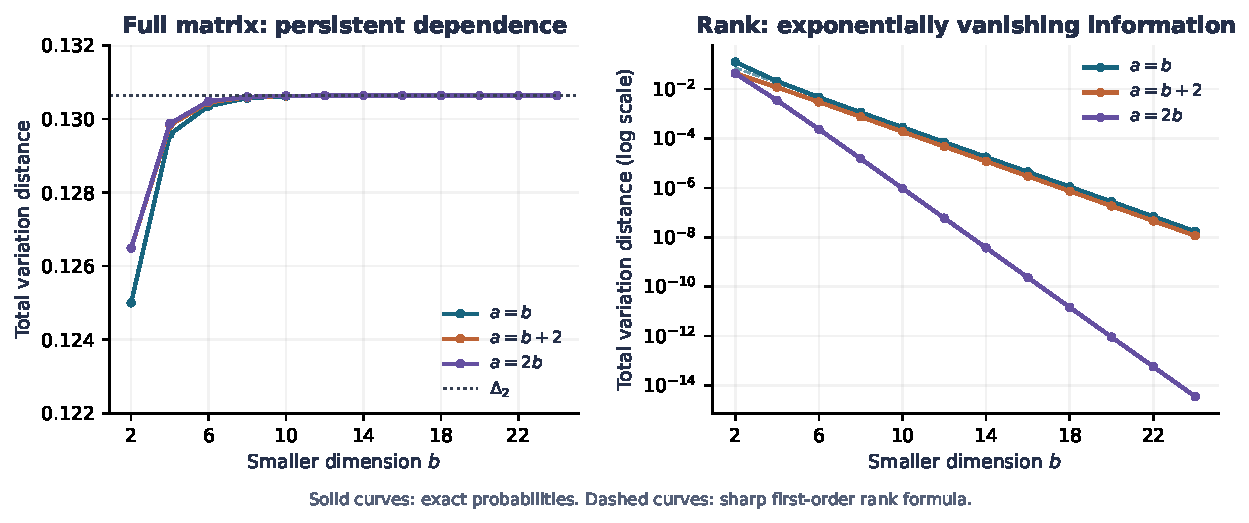
\includegraphics[width=\textwidth]{figures/symplectic_separation.pdf}
\caption{Uniform separation across shapes over $\mathbb F_2$. The complete matrix retains
a fixed testing advantage, while rank alone loses information exponentially in the larger dimension.
The dashed curves on the right are the proved first-order formula, not fitted regressions.}
\label{fig:separation}
\end{figure}

The data files retain the exact-enumeration receipts, high-precision comparison values, and
scaled remainders. Decimal evaluations use $150$ digits and $160$ factors of the infinite products.
The observed scaled remainders are evidence of agreement with the formulas; their finite maxima
are not asserted to be universal bounds. Both the main paper and the companion filter note
contain human-readable proofs. This packet contains no newly kernel-checked Lean formalization.


\begin{thebibliography}{9}
\raggedright

\bibitem{ProveIt}
Vladimir Reshetnikov, \emph{ProveIt: Beyond the Riemann hypothesis for Dirichlet $L$-functions: consequences, transfers and limits}, research repository, pinned commit
\texttt{497c1844e71393df41914f5b783d5dc9a618eb61}, inspected November 27, 2026.
Section on spanning, frames, auxiliary characters and matrix statistics.
\href{https://github.com/VladimirReshetnikov/ProveIt/blob/497c1844e71393df41914f5b783d5dc9a618eb61/Analysis/GeneralizedRiemannHypothesis/Article/sections/spn.tex}{Pinned section source}.
The article describes itself as a consolidation of delivered reports; our use of its finite formulas is supported by the proofs reproduced here.

\bibitem{FulmanGoldstein}
Jason Fulman and Larry Goldstein, \emph{Stein's method and the rank distribution of random matrices over finite fields}, Annals of Probability \textbf{43} (2015), no.~3, 1274--1314.
\href{https://doi.org/10.1214/13-AOP889}{doi:10.1214/13-AOP889};
\href{https://arxiv.org/abs/1211.0504}{arXiv:1211.0504}.

\bibitem{DeBoeckVanDeVoorde}
Maarten De Boeck and Geertrui Van de Voorde, \emph{Anzahl theorems for trivially intersecting subspaces generating a non-singular subspace I: symplectic and hermitian forms}, Linear Algebra and its Applications \textbf{699} (2024), 367--402.
\href{https://doi.org/10.1016/j.laa.2024.07.004}{doi:10.1016/j.laa.2024.07.004};
\href{https://arxiv.org/abs/2407.07486}{arXiv:2407.07486}.

\end{thebibliography}

\end{document}
